\chapter{Theoretical Background in Magnetic Resonance}
\section{Theory of Magnetic Resonance}
We will discus classical and quantum mechanical theory of magnetic resonance and spin dynamics in this chapter. Phenomenological Bloch equations and importance of motional effects on the spectral profiles will be covered as well.
\subsection{Energy Splitting and Bloch Equations}\label{blochsection}
In Nuclear Magnetic Resonance (NMR) atomic nuclei or unpaired electrons in Electron Paramagnetic Resonance (EPR) in strong applied magnetic field behave like a compass needle experiencing a torque tending to align its dipole moment in the direction of the field. Macroscopically model can be studied as system of N identical distinguishable and mutually non-interacting dipoles whose population ratio can be determined in terms of Boltzmann distribution~\cite{pathria}. Each individual dipole can be well described in terms of classical mechanics as motion of gyroscope in gravitational. Precise derivation and description can of phenomena can be found in any standard classical mechanics textbook like Goldstein~\cite{gold}. Torque of such "gyroscope" can be written in terms of magnetization $\vec{M}$ and applied magnetic field $\vec{B}$:
\begin{equation}\label{eq:torque}
\vec{\tau}=\vec{M}\times\vec{B}
\end{equation}
Motion of the magnetic moment can be described as following: 
\begin{equation}\label{eq:torque2}
\frac{d\vec{M}}{dt}=\gamma\vec{M}\times\vec{B}
\end{equation}
Where magnetic ratio $\gamma$ defines the ratio of a particle magnetic dipole moment to its angular momentum.\\*
Applied magnetic field creates interaction energy of the unpaired electron and known as Zeeman interaction: 
\begin{equation}\label{eq:1}
E = - \vec{\mu}\cdot \vec{B}
\end{equation}  
We can relate magnetic moment and angular momentum in terms of classical mechanics as following: 
\begin{equation}\label{eq:2}
\vec{\mu}=\gamma \vec{J}
\end{equation}
$\vec{J}$ is related to quantum mechanical dimensionless nuclear spin operator by the form $\hbar\hat{I}$ and in terms of EPR $I$ replaced by $S$ which acts on the electron spin states rather then nuclear spin states. Taking magnetic field $B_0$ is defined along z-axis allowed energies from Eq.\ref{eq:1} can be found as:
\begin{equation}\label{eq:3}
E=-\gamma\hbar S_z B_0=-\gamma\hbar m_S B_0
\end{equation} 
Where $S_z$ is a net spin of electron in $z$ direction and $m_S$ descirbes its eigenvalues. \\*
For example consider nitrooxide radical that has a single unpaired electron with spin $S=1/2$  and therefore two quantum spin states $m_S=\pm1/2$. Energy difference between higher and lower states can be calculated as:
\begin{equation}\label{eq:4}
\Delta E=\hbar \gamma B_0=\hbar \omega_0 \rightarrow \omega_0=\gamma B_0
\end{equation} 
For better understanding we can can schematically represent energy level split as a diagram that is shown on Figure \ref{figure:zeeman}. It is also useful sometimes to rewrite Eq.\ref{eq:4} by introducing electronic positive $g$ factor and Bohr magneton $\mu_{\beta}$. 
\begin{figure}[h!]
\begin{center}
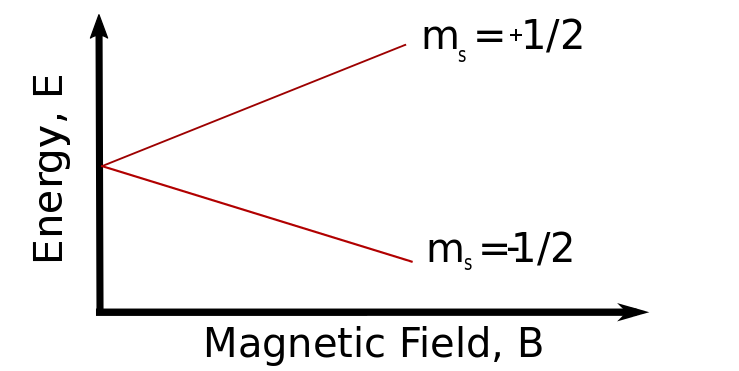
\includegraphics[width=0.7\textwidth]{figures/chap1/zems.png}
\caption{The effect of an a external magnetic field upon the energy of an electron and
the transition in induced by an a electromagnetic field for $S=\frac{1}{2}$ system in applied magnetic field $\vec B$}
\label{figure:zeeman}
\end{center}
\end{figure}
\begin{equation}\label{eq:5}
\hbar \omega_0=g\mu_{\beta}B_0 \rightarrow \omega_0=\frac{g\mu_{\beta}}{\hbar}B_0
\end{equation} 
$g$ factor carries important spectroscopic information and can be expressed as an anisotropic second rank tensor. We will cover more details on $g$ tensor in subsection 2.1.3.\\*
Meanwhile Equations \ref{eq:4} and \ref{eq:5} give a fundamental resonance condition and $\omega_0$ is known as Larmor frequency. In fact similar solution can be derived from the classical prospective as well. In 1946 Felix Bloch was the first who postulated time evolution of paramagnet "bulk" magnetization. Bloch was the first to explain magnetization of liquid samples by introducing inhomogeneity of the applied magnetic field. 
\begin{figure}[h]
\begin{center}
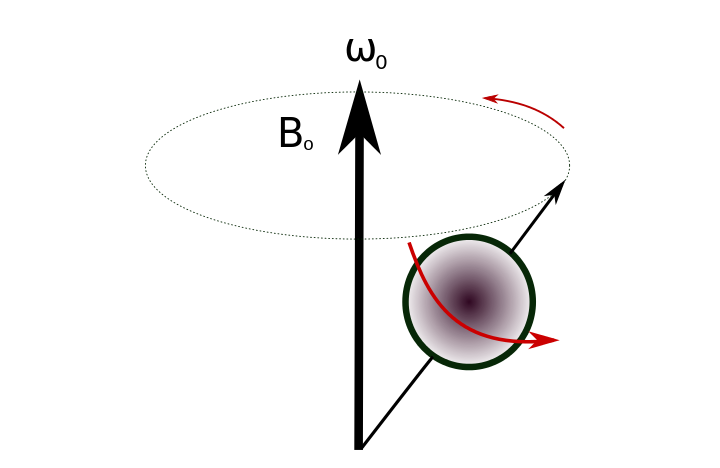
\includegraphics[scale=0.5]{figures/chap1/prec.png}
\caption{Magnetic moment precession in a constant magnetic field.}
\end{center}
\end{figure}

\begin{subequations}\label{eq:bloch}
\begin{align}
\frac{dM_x(t)}{dt}& =\gamma(M_y(t)B_z(t)-M_z(t)B_y(t))-\frac{M_x(t)}{T_2} \\
\frac{dM_y(t)}{dt}& =\gamma(M_z(t)B_x(t)-M_x(t)B_z(t))-\frac{M_y(t)}{T_2} \\
\frac{dM_z(t)}{dt} & =\gamma(M_x(t)B_y(t)-M_y(t)B_x(t))-\frac{M_z(t)-M_0}{T_1} 
\end{align}
\end{subequations}
Taking a step back to macro level. Interactions of unpaired electron spins with the environment in random and complicated fashion lead to thermal equilibrium defined by Boltzmann factor. In other words if number of nuclear or electron spins pointing up or down defined as $N_{\uparrow}$ and $N_{\downarrow}$ population ratio defined as follows:
\begin{equation}\label{eq:8}
\frac{N_{\downarrow}}{N_{\uparrow}}=exp(-\Delta E/k_{b}T)
\end{equation}
Where $k_b$ is a Boltzmann constant and $T$ is a sample temperature. This interactions lead to known as spin-lattice relaxation mechanism defined by longitudinal relaxation time $T_1$. 
On other hand various interactions between spins will not directly affect population ratio but will tend to cause transverse magnetization to decay and mechanism is known as spin-spin relaxation and characterized by time constant $T_{2}$. \\*
Effective magnetic field $B_{eff}$ due to preceding inhomogeneity can be written as following:
\begin{equation}\label{eq:inhomog2}
B_{eff}=B_0+B_1(t)
\end{equation}
Additional time-dependent field is added. In order to eliminate time dependence in fluctuating magnetic fields appropriate coordinate system should be chosen. In the rotating frame fixed static field has an additional term of $\frac{\omega_0}{\gamma}$ thus in the rotating frame
\begin{equation}\label{eq:inhomog}
B_{eff}=(B_0+\frac{\omega_0}{\gamma})\vec{i}+B_1\vec{j}
\end{equation}
As example construction of Bloch equations for low $B_1$ to avoid saturation effects can be easily shown. Choosing unit vector $i$ to be in parallel with $z(\hat{z})$ and direction of oscillating field in laboratory frame defined in $x$ direction($\hat{x}$)  and define 
 \begin{equation}\label{eq:inhomog3}
B_1=-\frac{\omega_1}{\gamma}2\cos\omega t\hat{x}
\end{equation}
In the rotating frame Bloch equations from \eqref{eq:bloch} can be rewritten as: 
\begin{subequations}\label{eq:bloch2}
\begin{align}
\frac{dM_x(t)}{dt}& =\Delta\omega M_y-\frac{M_x(t)}{T_2} \\
\frac{dM_y(t)}{dt}& =-\Delta\omega M_x-\frac{M_y(t)}{T_2}-\omega_1M_z \\
\frac{dM_z(t)}{dt} & =\omega_1M_y-\frac{M_z(t)-M_0}{T_1} 
\end{align}
\end{subequations}
Difference between Larmour and irradiation frequencies gives the energy absorption in the system and defined as $\Delta\omega=\omega-\omega_0$ and conditionally it defines resonance phenomenon. Evolution of net magnetization of the sample can be generalized and predicted in terms of Bloch equations solving it with the specific to the system constraints. For high field experiments when $B_0 \sim B_1$ or including line saturation, harmonic generation, multiquantum transitions and etc. solution becomes not trivial. 
\subsection{Density Matrix}\label{densitymatrixsubsection} 
SENTENCE ON HOW WE CAME UP TO THIS in GAMILEL
We can describe magnetization quantum mechanically using expectation value nuclear or spin angular momentum quantum operators. To find time evolution of the sample magnetization the density matrix approach should be used.\\* 
To begin with lets quicly refresh basic concepts of quantum mechanics. We start with composition of the wave function of other two: 
\begin{equation}\label{eq:10}
|\psi_{total}\rangle=|\psi_{system}\rangle|\psi_{enviroment}\rangle=\sum_{i,j} c_{i,j}|\psi_{i(system)}\rangle|\psi_{j(enviroment)}\rangle
\end{equation}
The expectation value of an observable that operates only on the system ($S,I$ spin operators) can be written in complete set of basis states as:
\begin{equation}\label{eq:11}
\langle A \rangle=\sum_{i,j} c_{i,j}^*c_{k,l}^*\langle \theta_{(j(env))}|\langle \phi _{i(sys)}|A|\phi_{k(sys)}\rangle|\theta_{l(env)}\rangle=\sum_{i,k}\rho_{k,i}A_{i,k}
\end{equation}
Where $\rho$ is known as density matrix and coefficients $c_{i,j}$ are modeling a coupling that provides characterization of the state of the ensemble of quantum systems. 
Density matrix is hermitian thus it can be diagonalized and written as following: 
\begin{equation}\label{eq:13}
\hat{\rho}=\sum_{ij}\rho_{ij}|\phi_i\rangle\langle \phi_j|
\end{equation} 
Where $\rho_{ij}$ are eigenvalues. Using Schroedinger equation we can writte: 
\begin{equation}\label{eq:14}
\frac{\partial \hat{\rho}}{\partial t}=\frac{1}{i\hbar}\sum_{ij}\rho_{ij}\Big[\Big(\frac{\partial}{\partial t}|\phi_i\rangle\Big)\langle \phi_j|+|\phi_i\rangle\ \Big[\Big(\frac{\partial}{\partial t}\langle \phi_j|\Big)\Big]
\end{equation} 
Or recalling Schroedinger Equation from childhood memories can be rewritten as: 
 \begin{equation}\label{eq:15}
\frac{\partial \hat{\rho}}{\partial t}=\frac{1}{i\hbar}[\hat{H},\hat{\rho}]
\end{equation} 
In such motion observables are time independent and density operator is time-dependent. 
This equation can be directly solved in vector space known as Liouville where $\rho$ can be represented as vector. Eq.\ref{eq:15} can be rewritten as:
 \begin{equation}\label{eq:16}
\frac{d\rho_{ij}}{dt}=\frac{1}{i\hbar}\sum_{k,l}(H_{ik}\delta_{lj}-\delta_{ik}H_{jl}^T)\rho_{kl}=-\frac{i}{\hbar}\sum_{k,l}\mathcal{L}_{ij,kl}\rho_{kl}
\end{equation} 
Where $\mathcal{L}$ defines the Liouville super-operator which operates on Hilbert space operators. In this notation each matrix element is labeled by two indexes. Such unusual notation will later bring a computational simplification for Magnetic Resonance computations. 
using Kroenecker tensor product super-operator can be written as 
\begin{equation}\label{eq:17}
\hat{\mathcal{L}}=\hat{H}\otimes\hat{I}-\hat{I}\otimes\hat{H}^{T}
\end{equation} 
Where $\hat{I}$ is a unit matrix of rank of $\hat{H}$
As simple example for nuclei or spin 1/2 operator time-dependent Hamiltonian can be written as: 
\begin{equation}\label{eq:18}
\hat{H} = \begin{bmatrix}
       0 & f^*           \\[0.3em]
       f & 0 \\[0.3em]
     \end{bmatrix}
\end{equation}
Liouville supermatrix is following: 
\begin{equation}\label{eq:19}
\hat{\mathcal{L}} = \begin{bmatrix}
       0 & -f & f^* & 0          \\[0.3em]
       -f^* & 0 & 0 & f^* \\[0.3em]
       f & 0 & 0 & -f \\[0.3em]
       0 & f & -f^* & 0 
     \end{bmatrix}
\end{equation}
The ordering of the rows and columns of $\hat{\mathcal{L}}$ are all equivalent up to a unitary transformation, but the ordering of the rows and columns of $\hat{\mathcal{L}}$ arising from the definition of the Kronecker tensor product is perhaps the easiest to follow. As example, the $f=\hat{\mathcal{L}_{1/2,1/2;-1/2,1/2}}$ matrix element arises from conjugate of $f$ as $f^*=\hat{\mathcal{H}_{1/2,-1/2;}\delta_{1/2,1/2}}=$. Another example that is  for calculation is spin 1 system. Both $g$ and $f$ here are some time-dependent functions yet to be determined by the interacting system and its surroundings interraction. Assuming that Hamiltonian given as: 
\begin{equation}\label{eq:hamliv}
\hat{\mathcal{H}} = \begin{bmatrix}
       g & f^* & 0 \\[0.3em]
       f & 0 & f^* \\[0.3em]
       0 & f & -g \\[0.3em]
     \end{bmatrix}
\end{equation}
Corresponding Liouville matrix has a following form: 
\begin{equation}\label{spinoneliv}
\hat{\mathcal{L}} = \begin{bmatrix}
       0 & -f & 0 & f^* &0 & 0 & 0 & 0 & 0         \\[0.3em]
       -f* & g  & -f   & 0 &f^* & 0  & 0   & 0 & 0         \\[0.3em]
       0 & -f^*  & 2g   & 0 &0 & f^*  & 0   & 0 & 0         \\[0.3em]
       f & 0  & 0   & -g &-f & 0  & f^*   & 0 & 0         \\[0.3em]
       0 & f  & 0   & -f^* &0 & -f  & 0   & f^* & 0         \\[0.3em]
       0 & 0  & f   & 0 &-f^* & g  & 0   & 0 & f^*         \\[0.3em]
       0 & 0  & 0   & f &0 & 0  & -2g   & -f & 0         \\[0.3em]
       0 & 0  & 0   & 0 &f & 0  & -f^*   & -g & f-         \\[0.3em]
       0 & 0  & 0   & 0 &0 & f  & 0   & -f^* & 0         \\[0.3em]
     \end{bmatrix}
\end{equation}
There are different approaches on algorithm of Liouville matrix construction that can be useful if corresponding interacting quantum mechanical system has spin greater then 1 and construction by hand can be tedious. More details and discussion can be found in Gamilel~\cite{gam} first chapters and suggested for the reader.   
\subsection{The g-tensor}\label{gtensorsection}
In crystaline and liquid systems EPR spectra may be dependent on the orientation of the sample relative to applied magnetic field $B_0$. This phenomena is also known as spectrum anistopy. Recall Zeeman Hamiltonian term for electron spin as: 
\begin{equation}\label{eq:20}
\mathcal{\hat{H}}=\beta \vec{B}\cdot g \cdot \hat{S}
\end{equation} 
In Eq.\ref{eq:20} $g$ factor is represented as 2-nd rank tensor. Anisotropy of the $g$ factor arises from spin-orbit coupling between the ground state and excited states of unpaired electrons. If applied magnetic field is chosen in the direction of cosines$(\hat{i},\hat{j},\hat{k})$ in the laboratory frame with $S_z$ to be diagonal a simple example is to construct Hamiltonian matrix and define its eigenvalues for $S=1/2$:

\begin{equation}\label{eq:21}
\mathcal{H} = \begin{bmatrix}
       \frac{1}{2}\beta B_0( \hat{i}g_{xz}+\hat{j}g_{yz}+\hat{k}g_{zz}) & \frac{1}{2}\beta B_0( \hat{i}g_{xx}+\hat{j}g_{xy}+\hat{k}g_{xz})          \\[0.3em]
  & -i(\hat{i}g_{xy}+\hat{j}g_{yy}+\hat{k}g_{yz}) \\[0.3em]      
       \frac{1}{2}\beta B_0( ig_{xx}+jg_{xy}+kg_{xz})  &  -\frac{1}{2}\beta B_0( \hat{i}g_{xz}+\hat{j}g_{yz}+\hat{k}g_{zz}) \\[0.3em]
        -i(\hat{i}g_{xy}+\hat{j}g_{yy}+\hat{k}g_{yz})  & \\[0.3em]
     \end{bmatrix}
\end{equation}
Values of the $g$ factor matrix can be found from difference between eigenvalues of the Hamiltonian matrix in Eq.\ref{eq:21}. Thus generalized form can be written as: 
\begin{equation}\label{eq:gtengeneral}
\begin{array} {lcl} &g^2& = g_{xx}^2\sin^2\theta\cos^2\phi+2g_{xy}^2\sin^2\theta cos\theta+g_{yy}^2sin^2\theta\\ & + & g_{yy}\sin^2\theta\sin^2\phi+2g_{xz}\cos\theta\sin\theta\cos\phi\\ & + & 2g_{yz}\cos\theta\sin\theta\sin\phi+g_{zz}\cos^2\theta \end{array}
\end{equation}
Matrix elements can be determined impericall by the finite number of the sample rotations in applied magnetic fields in $xy,yz$ and $xz$ planes. For $xz$ plane $\theta$ is an angle between magnetic field and $z$ axis and $\phi=0$. Thus $g$ tensor has a following form:  
\begin{equation}\label{eq:22}
g^2=g_{xx}^2\sin^2\theta+2g_{xz}^2\sin^2\theta \cos\theta+g_{zz}^2\cos^2\theta
\end{equation} 
When $yz$ plane is rotated around $\phi=90^{\circ}$:
\begin{equation}\label{eq:newone22}
g^2=g_{yy}^2\sin^2\theta+2g_{yz}^2\sin\theta cos\phi+g_{zz}^2sin^2\theta\cos\phi\sin\phi
\end{equation} 
And for the $xy$ plane $\theta=90^{\circ}$:
\begin{equation}\label{eq:newone221}
g^2=g_{xx}^2cos^2\phi+2g_{xy}^2\sin\phi\cos\phi+g_{yy}^2\sin^2\phi
\end{equation} 
In order to obtain unique values of the $g$ tensor three measurements in each plane should be performed. For example if $\theta=0$ and $\theta=90^{\circ}$ one can obtain $g^2_{xx}$ and $g^2_{zz}$. Matrix $g^2$ can be diagonalized by casting direction of cosines which define molecular frame to laboratory frame. Hamiltonian in principal axis of $g$ tensor can be written as: 
\begin{equation}\label{eq:princham}
\mathcal{H}=\vec{B}\cdot \begin{bmatrix} g_{xx} & 0 & 0 \\ 0 & g_{yy} & 0\\ 0 & 0 & g_{zz}\end{bmatrix}\cdot \hat{S}
\end{equation}   
Matrix calculation were reduced from finding nine elements to three which is enough to obtain important geometrical and quantum mechanical information on the species. For symmetric magnetic samples axis coincide with principal axis of $g$ tensor and symmetry planes are usually perpendicular to them. For molecules like eclipsed ethane with low symmetry the principal axes orthogonal to each other can point to arbitrary direction specified by local magnetic field.\\*
There are in general three groups of symmetry: cubic, uniaxial and rhombic and presented of Fig.\ref{figure:gsym}. For the cubic symmetry principal values of $g$ tensor are equal to each other $g_{xx}=g_{yy}=g_{zz}$ so that anisotropy in EPR spectra vanishes and absorpion spectrum presented as one Lorentzian lineFig.\ref{figure:gsym}(a). Uniaxial case is when $g_{xx}=g_{yy}<g_{zz}$ or $g_{xx}=g_{yy}>g_{zz}$ shape of the absorption and derivative spectrum has a step sides Fig.\ref{figure:gsym}(b),(c). Rhombic symmetry Fig.\ref{figure:gsym}(d) is given when $g_{xx}\neq g_{yy}\neq g_{zz}$ and typical for nitrooxide free radicals that are of interest to our research and this particular thesis. 
\begin{figure}[h!]
\begin{center}
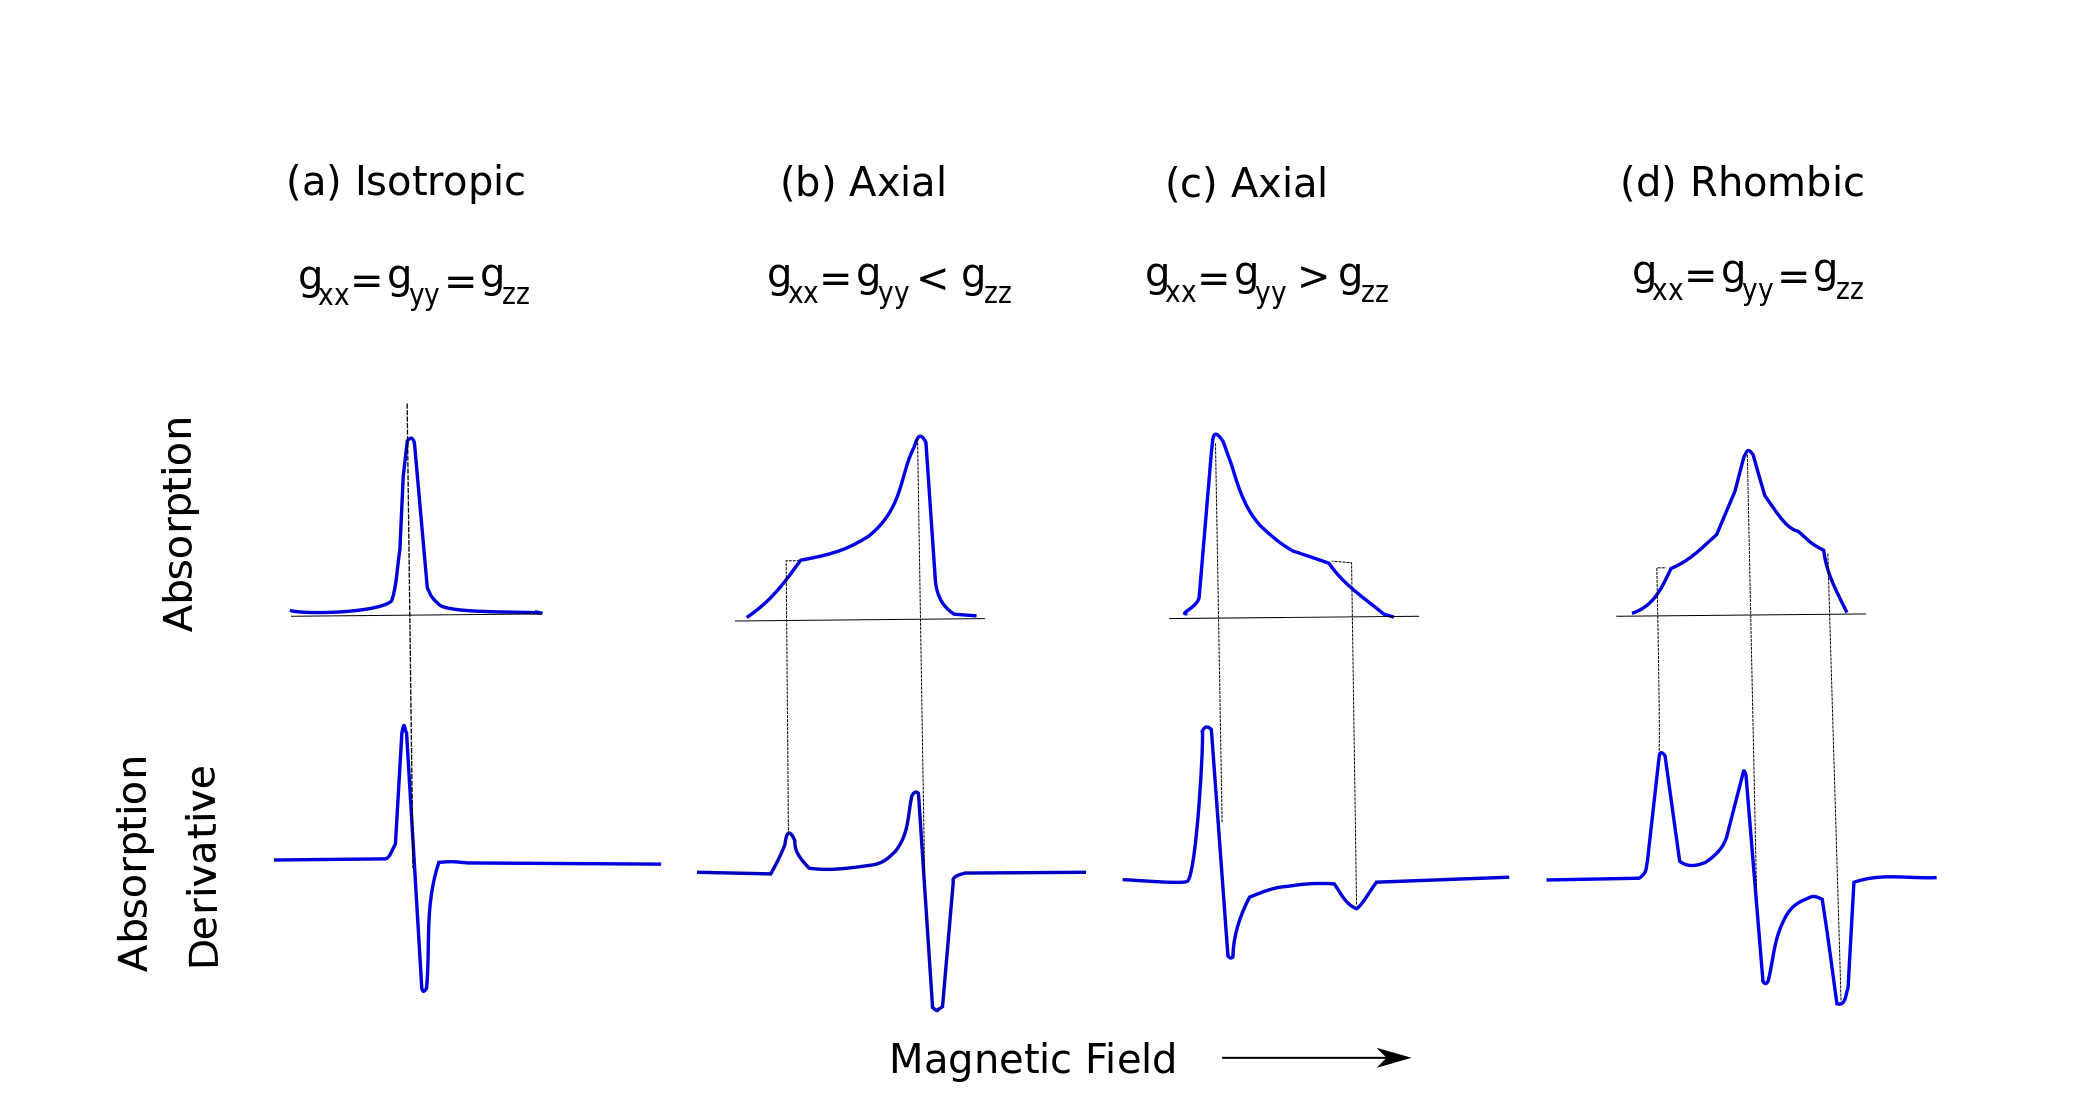
\includegraphics[width=1\textwidth]{figures/chap1/gten1.png}
\caption{Absorpton lineshape and its derrivative for randomly oriented spin system with (a) cubic(isotropic) symmetry; (b),(c) uniaxial symmetry and (d) rhombic symmetry.}
\label{figure:gsym}
\end{center}
\end{figure}
\\*
Additionally deviations from electron $g_e$ arise from spin-orbit coupling. Consider to rewritte $g$ tensor by adding supplementary term as:
\begin{equation}\label{eq:gtenelec}
\pmb{g}=g_e\hat1+\Delta \pmb{g}_{SO/OZ}+\Delta\pmb{g}_{RMC}+\Delta\pmb{g}_{GC}
\end{equation} 
First term is a free electron $g$-factor and its value is approximatelly $g_e=2.0023...$ multiplied by the identity matrix. Second term represents spin orbital/orbital-Zeeman coupling, second term is known as "mass-velocity" correction and third term is a gauge correction they are both diamagnetic and much smaller compared to the first term. In order to find spin-orbit/orbial-Zeeman term from second order perturbation theory excited states $|n\rangle$ and ground states $|0\rangle$ should be determined for quantum mechanical system. Shift can be written as~\cite{thesis1}:  
\begin{equation}\label{eq:zeemanparamagn}
\Delta \pmb{g}_{SO/OZ}=\frac{2g_e\beta_e^3}{\hbar^2k_0c^2\langle S_z\rangle}\sum_N Z_N\sum_n\Bigg[ \frac{\langle0|\hat{\pmb{O}_1}|n\rangle\langle n|\hat{\pmb{O}_2}|0\rangle}{E_0^{(0)}-E_n^{(0)}}+c.c\Bigg]
\end{equation} 
Here $N$ is order of nuclei and $"c.c"$ are complex conjugate of spin-orbit coupling integrals.For 1-electron coupling integral is given as:
\begin{equation}\label{eq:oneel1}
\langle 0|\sum_i\frac{1}{r^3_{iN}}\times(\hat1_{iN})_us_{iz}|n\rangle\langle n|\sum_j(\hat1_{iN})_v|0\rangle
\end{equation}
And integral for 2-electron coupling can be written as:
\begin{equation}\label{eq:oneel2}
\langle 0|\sum_{ij}[\pmb{r}_{ij}\times(\nabla_i-2\nabla_j)]_us_{jz}|n\rangle\langle n|\sum_j(\pmb{r}_k\times\nabla_k)_v|0\rangle
\end{equation}
Where summation is done over all orbitals $(i,j)$ and $u,v$ are the Cartesian axises. Thus we have and complete udnerstanding of the the $g$-tensor anysotropy by now. 
\subsection{A-tensor}\label{atensorsection}
The interaction between spin of unpaired electron with local magnetic fields which are product of spin of nuclei in the molecule where electron is located can lead to additional spectral lines. Electron and nuclear spins are quantized thus number of lines for a single nuclei can be found as $2I+1$ and they are clustered around major Zeeman energy levels. This interaction is known as Nuclear Hyperfine interaction. Separation between this additional lines determined by the hyperfine coupling constant. Hamiltonian for hyperfine interaction can be written~\cite{nordio}: 
\begin{equation}\label{eq:23}
\mathcal{\hat{H}}_{hf}=-g_e\beta_eg_N\beta_N\Big[\frac{(\hat{I}\cdot \hat{S})r^2-3(\hat{I}\cdot\vec{r})(\hat{S}\cdot\vec{r})}{r^5}-\frac{8\pi}{3}(\hat{I}\cdot\hat{S})\delta(\vec{r})\Big]
\end{equation} 
Where $\vec{r}$ is a electron-nucleus distance, $g_N$ and $\beta_N$ are nucleus $g$ factor and Bohr magneton respectively. First term represents dipolar coupling of electron to nucleus~\cite{car} and can be derived from interaction energy between an electron and nucleus that are located distance $r$ from each other so that quantum mechanical opartors will be simply replaced by corresponding magnetic magnetic moments. This term bring anisotropy and known as anisotropic part of the Hyperfine interaction. Second term known as Fermi contact coupling which is proportional to spin density at nucleus and represents isotropic interaction ~\cite{slich}. For the simplification anisotropy in a $g$ tensor was neglected. Eq.\ref{eq:23} can be also written as: 
\begin{equation}\label{eq:24}
\mathcal{\hat{H}}_{hf}= \mathcal{\hat{H}}_1+\mathcal{\hat{H}}_2=\hat{I}\cdot A'\cdot\hat{S}+a\hat{I}\cdot\hat{S}
\end{equation} 
$A'$ is anisotropic second rank tensor that is similarly defined as $g$ tensor. Expanding in terms of matrix elements and averaging over electron distribution:
\begin{equation}\label{eq:25}
A'_{ij}= -g_e\beta_eg_n\beta_n\langle(r^2\delta_{ij}-3r_ir_j)r^{-5}\rangle
\end{equation} 
Where $i\rightarrow[x,y,z],j\rightarrow[x,y,z]$ are coordinates of electron in laboratory frame and point nucleus assume to be placed at the origin. For the contact interaction one can be obtained coupling constant assuming unpaired electron wave function $\psi(0)$ is known represents isotropic value:
\begin{equation}\label{eq:26}
a= \Big(\frac{8\pi}{3}\Big)g_e\beta_eg_N\beta_n\psi^2(0)
\end{equation}
$a$ is a rotation invariant thus it is namely known as isotropic part of hyperfine tensor. Taking to account both terms once can define in the lab-frame the Hyperfine Tensor as:  
\begin{equation}\label{eq:27}
A_{ij}=A'_{ij}+\delta_{ij}a
\end{equation} 
Anisotropic part is dominating over isotropic~\cite{griff} . Due to the fact that this interaction only occurs when the electron is inside the nucleus, only electrons in the s orbital exhibit this kind of interaction. All other orbitals (p,d,f) contain a node at the nucleus and can never have an electron at that node.\\* Principal components of anisotropic hyperfine  tensor $A$ can be find in a similar way as for $g$ tensor,
\begin{equation}\label{eq:atengeneral}
\begin{array} {lcl} &A^2& = A_{xx}^2\sin^2\theta\cos^2\phi+2A_{xy}^2\sin^2\theta cos\theta+A_{yy}^2sin^2\theta\\ & + & A_{yy}\sin^2\theta\sin^2\phi+2A_{xz}\cos\theta\sin\theta\cos\phi\\ & + & 2A_{yz}\cos\theta\sin\theta\sin\phi+A_{zz}\cos^2\theta \end{array}
\end{equation}
Effect of rhombic anisotropy will be treated in this work. 
\subsection{Rotations in Magnetic Resonance}\label{torationsection}
In previous sections discussing anisotropy of the Hamiltonians due to orientation dependence of sample relative to the strong applied magnetic field. Sometimes each specific parts of the Hamiltonian are defined in the different reference frames thus unified algorithm on gathering all frames together should be introduced.\\*  
For example applied magnetic field $\vec{B}$ is defined in Laboratory Frame(LF) and axis as was discussed previously is taken along z-axis. In complex samples such as liquids or membranes it is always an interest to introduce Directory Frame(DF) where usually z-axis is along restoring potentials and z and y-axis are coincide with the same axis in LF. DF is usually tilted from relative to the $\vec{B}$ by the angle $\psi$ which can be obtained by the set of Euler angles that transform LF to DF~\cite{rotat}~\cite{bmr}. Diffusion tensor is defined in the frame relative to the molecular orientations o Molecular Frame(MF). it is usually axial symmetric thus having any arbitary direction that can be fixed within Laboratory Frame by the specification of the second Euler angle~\cite{bmr} which is true in the limit of nitrooxide spin labelling line shape calculation. The last two frames are the principal frames of the $g$ and $A$-tensors which can be transformed to the MF and then to LF by the set of all three Euler angles. In most cases $g$ and $A$-tensors principal axes are coincide thus simplifying theoretical work for the line shape calculation. Diagram of all the frames is given at Fig.\ref{figure:rotat}
\begin{figure}[h]
\centering
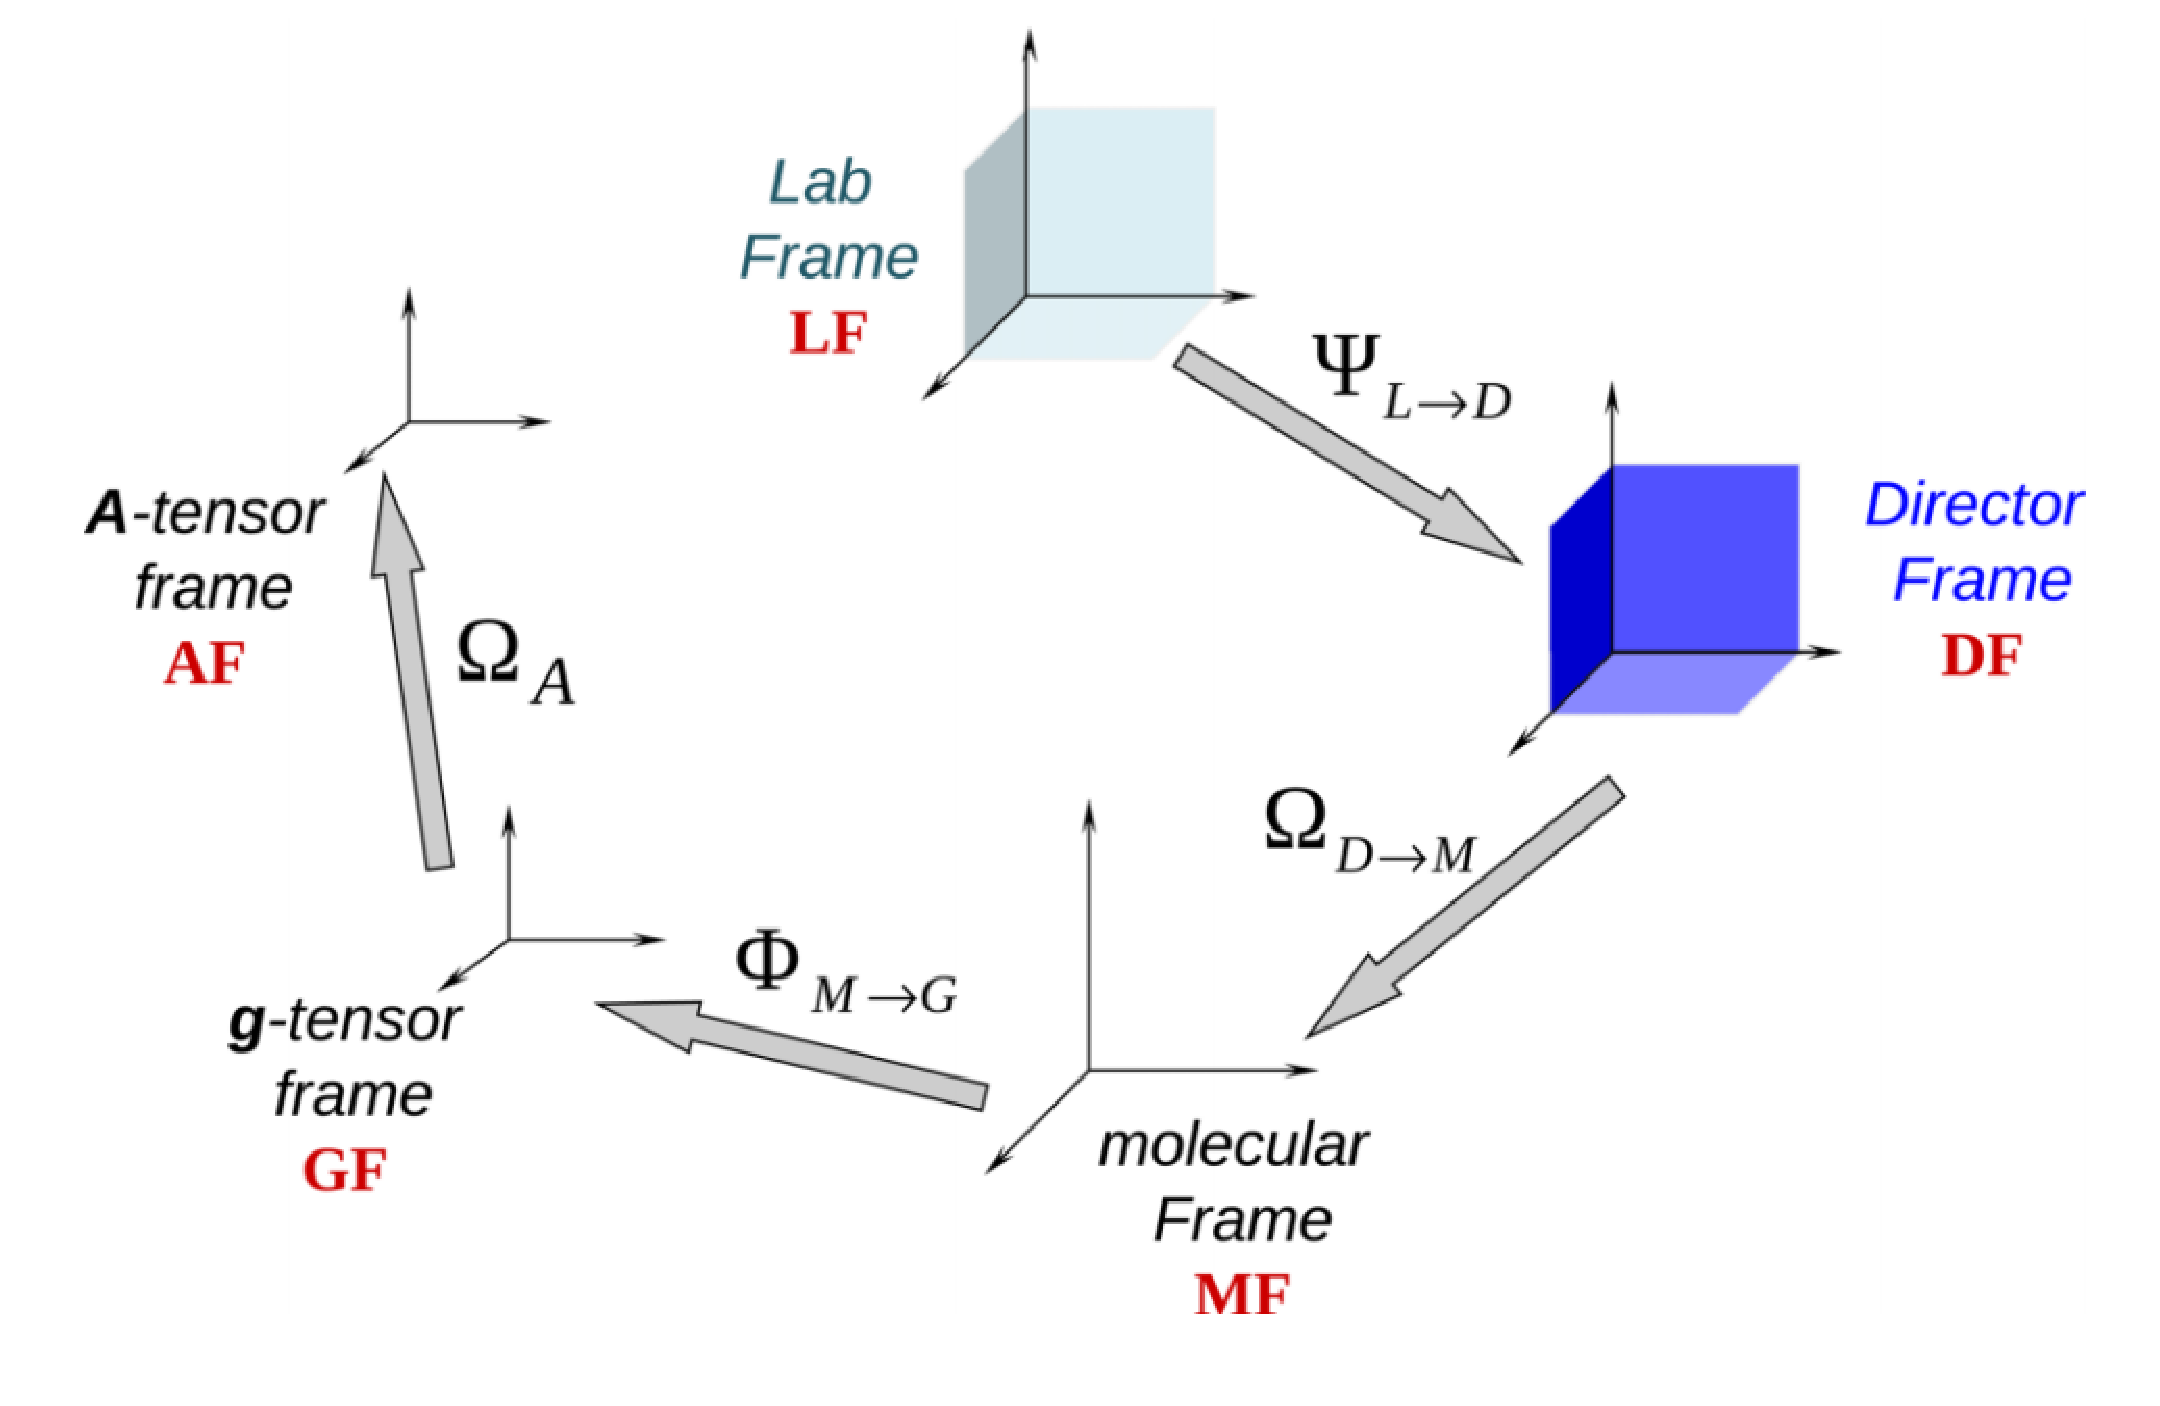
\includegraphics[width=0.7\textwidth]{figures/chap1/frames.eps}
\caption{Example of reference frames that define structural and dynamic properties of the spin-labelled molecules.~\cite{rotat}}
\label{figure:rotat}
\end{figure}
Starting with the detailed construction using Zeeman and Hyperfine interactions it will be shown the powerful use of tensor algebra in magnetic resonance theory:   
\begin{equation}\label{eq:39}
\mathcal{\hat{H}}_{eff}=\hat{S}\cdot g_S\cdot \vec{B}+\hat{S}\cdot A \cdot \hat{I}
\end{equation} 
Space part is represented by $g$ and $A$ tensors that are defined in their own and unique principal axis frames($P$)that are fixed to each other by the molecular frame~\cite{marina}. Magnetic field and spin operators as well as their product are defined in only in a static or laboratory frame. In order to compute EPR spectra or resonance frequencies both tensors have to be defined in the laboratory frame. Rotation of the $g$-tensor to lab frame schematically:  
\begin{equation}\label{eq:40}
 g_{S(P)}\xrightarrow{\textbf{R"}}g_{S(L)}
\end{equation}
Hyperfine tensor $A$ should then rotated into $g$-tensor principal axes and second rotation is done to laboratory frame axes or vice versa. 
\begin{equation}\label{eq:41}
  A_{P}\xrightarrow{\textbf{R'}}A_{g}\xrightarrow{\textbf{R"}}A_{L}
\end{equation}
Here $R', R"$ are rotational matrices that establish mutual orientation between $g$ and $A$ tensors and laboratory frame. There are two ways to treat such rotational transformations between frames. In the first way Cartesian tensors are rotated directly and in second way they are decomposed into irreducible spherical tensor(ISTO) components which are rotating independently and combined back into transformed Cartesian tensor. Spherical tensor operators in three dimensional space have more symmetry features which makes them as more favourable method to use and even more obvious\cite{duer}. The individual spherical tensor components $T_{ml}$ of rank $l$ are given as,     
\begin{equation}\label{eq:42}
  T^{R}_{ml}=\sum_{m'=-l}^lT_{mm'}\mathcal{D}^{(l)}_{mm'}\Omega(\alpha,\beta,\gamma)
\end{equation}
This is analogous to angular momentum basis ket transformation.Rotations in 3-D parametrized by set of Euler equations $\Omega(\alpha,\beta,\gamma)$ transforming stationary $Oxyz$ to a rotational $OXYZ$. Euler angles transformation define orientation of an object in a body-fixed frame to a spaced-fixed of an object. Such transformation is defined by active rotation matrix\cite{bouten}\cite{mul}: 
\begin{figure}[h]
\centering
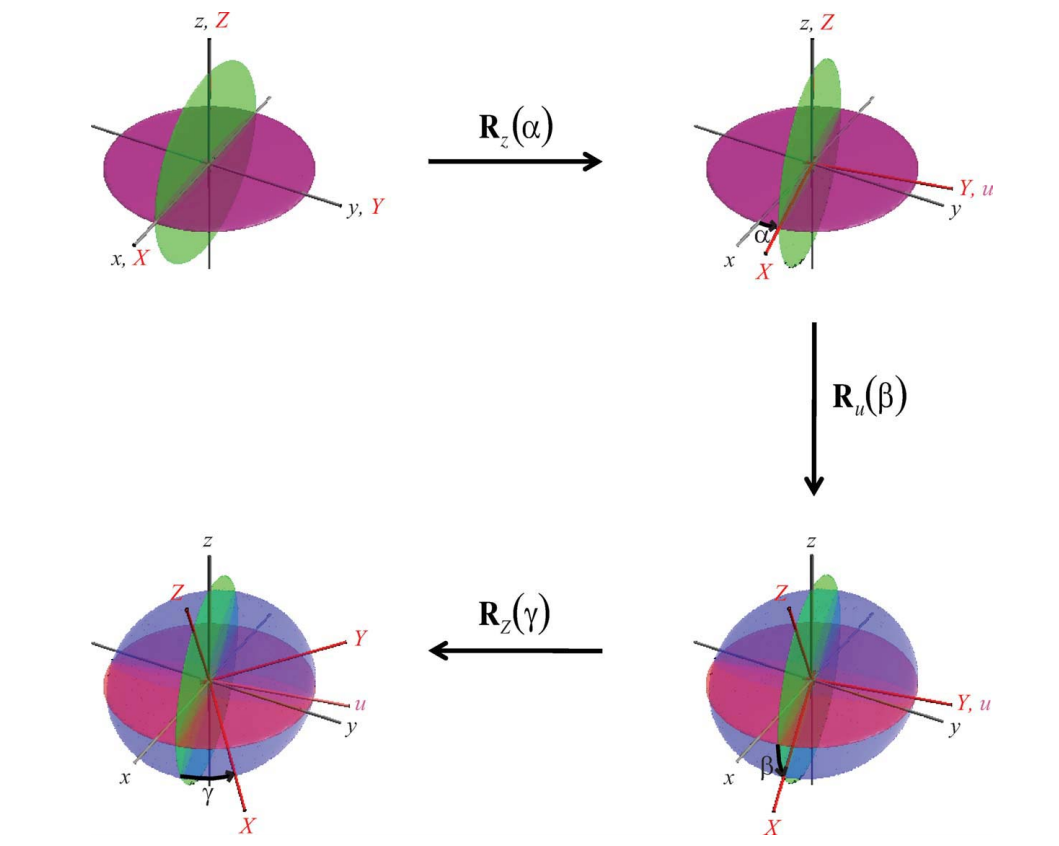
\includegraphics[width=0.7\textwidth]{figures/chap1/rot.png}
\caption{Figure from \cite{mul}}
\end{figure}
\begin{equation}\label{eq:43}
\textbf{R}_A(\alpha,\beta,\gamma) = \begin{bmatrix}
       \cos\alpha \cos\beta \cos\gamma-\sin\alpha \sin\gamma & -\cos\alpha \cos\beta \sin\gamma-\sin\alpha \cos\gamma & \cos\alpha\sin\beta         \\[0.3em]
       \sin\alpha \cos\beta \cos\gamma-\cos\alpha \sin\gamma & -\sin\alpha \cos\beta \sin\gamma-\cos\alpha \cos\gamma & \sin\alpha\sin\beta  \\[0.3em]
       -\sin \beta \cos\gamma & \sin \beta \sin\gamma & \cos \beta
     \end{bmatrix}     
\end{equation}
Transformation back from spaced-fixed frame to body-fixed frame defined by passive rotation transformation matrix $\textbf{R}_P$ and related to active as $\textbf{R}_P(\alpha,\beta,\gamma)=\textbf{R}_A^{-1}(\alpha,\beta,\gamma)$. \\*
Elements $\mathcal{D}_{m,m'}^l$ are known as Wiegner rotation matrix elements and they define expectation values of rotation operator for all magnetic quantum numbers $m$ and $m'$ of the angular momentum $l$ generating rotations~\cite{tomog}: 
\begin{equation}\label{eq:44}
\mathcal{D}_{m,m'}^l=\langle \mathcal{O}(\alpha,\beta,\gamma)\rangle= \langle l,m'|exp(-i\alpha I_x)exp(-i\beta I_y)exp(-i\gamma I_z)|l,m\rangle
\end{equation}
Exponential values with $I_z$ operator can be expanded in Taylor series and evaluated in terms of eigenvalues $m,m'$\cite{brink}. Eq.\ref{eq:44} can be rewritten as:
\begin{equation}\label{eq:45}
\mathcal{D}_{m,m'}^l=exp(-i\alpha I_x)d_{m',m}^{(l)}exp(-i\gamma I_z)
\end{equation}
Where $d_{m',m}^{(l)}$ are reduced Wigner rotation matrix elements. They are real functions and values up to $l=2$ values are given in table \ref{tab:wigner}. Presented table below extremely useful when constructing the full Hamiltonian. 
\begin{table}
\begin{center}
    \begin{tabular}{  l | l }
    \hline
    $d^{l}_{m,m'}$ for $l=1/2,1$ & $d^{l}_{m,m'}$ for $l=2$ \\ \hline
    $d^{1/2}_{1/2,1/2}=d^{1/2}_{-1/2,-1/2}=\cos\frac{\beta}{2}$ & $d^{2}_{2,2}=d^{2}_{-2,-2}=\cos^4\frac{\beta}{2}$ \\
    $d^{1/2}_{-1/2,1/2}=-d^{1/2}_{1/2,-1/2}=\sin\frac{\beta}{2}$ & $\begin{array} {lcl} d^{2}_{2,1} & = & d^{2}_{1,2}=-d^{2}_{1,2} \\ & = & d^{2}_{-1,-2}=-\frac{1}{2}\sin\beta(1+\cos\beta) \end{array}$  \\ 
    $d^{1}_{1,1}=d^{1}_{-1,-1}=\cos^2\frac{\beta}{2}$ & $\begin{array} {lcl} d^{2}_{2,0} & = & d^{2}_{0,2}=-d^{2}_{-2,0} \\ & = & d^{2}_{0,-2}=\sqrt\frac{3}{8}\sin^2\beta \end{array}$ \\ 
    $d^{1}_{1,-1}=d^{1}_{-1,1}=\sin^2\frac{\beta}{2}$ & $\begin{array} {lcl} d^{2}_{2,-1} & = & d^{2}_{1,-2}=-d^{2}_{-2,1} \\ & = & d^{2}_{-1,-2}=\frac{1}{2}\sin\beta(\cos\beta-1) \end{array}$ \\ 
   $\begin{array} {lcl} &d^{1}_{0,1}& =  d^{1}_{-1,0}=-d^{1}_{0,-1}\\ & = & -d^{1}_{1,0}=-\frac{1}{\sqrt{2}}\sin\beta \end{array}$ & $d^{2}_{2,-2}=d^{2}_{-2,2}=\sin^4\frac{\beta}{2}$ \\ 
    $d^{1}_{0,0}=\cos\beta$  & $\begin{array} {lcl} d^{2}_{1,1} & = & d^{2}_{-1,-1} \\ & = & \frac{1}{2}(2\cos\beta-1)(\cos\beta+1) \end{array}$\\ 
     $d^{0}_{0,0}=1$ & $\begin{array} {lcl} d^{2}_{1,-1} & = & d^{2}_{-1,1} \\ & = & \frac{1}{2}(2\cos\beta+1)(1-\cos\beta) \end{array}$ \\ 
      & $\begin{array} {lcl} d^{2}_{1,0} & = & d^{2}_{0,-1}=-d^{2}_{0,1} \\ & = & d^{2}_{-1,0}=-\sqrt\frac{3}{2}\sin\beta\cos\beta \end{array}$ \\ 
      & $d^{2}_{0,0}=\frac{1}{2}(3\cos^2\beta-1)$ \\ \hline
   
    \end{tabular} 
\end{center}
\caption{Algebraic expressions for Wigner rotation matrix elements}
  \label{tab:wigner}
 \end{table}
Hamiltonian is rank zero tensor and thus rotation invariant under coordinate transformation. Using the fact that spherical tensors of the same rank can be contracted the Hamiltonian for the system can be written as~\cite{nordio}:
\begin{equation}\label{eq:46}
  \mathcal{\hat{H}}=\sum_{(int)}\sum_{lm}(-1)^mF_{-m,(int)}^lA_{m,(int)}^l
\end{equation}
where $F_{-m,(int)}$ are components of irreducible spherical tensor describing nature of the interaction and 
$A_{m,(int)}^l$ describe spin operators depending on the type of interaction. $(int)$ decribes the type of interaction(zeeman, hyperfine, dipolar. etc.). 
\begin{equation}\label{eq:47}
  \mathcal{\hat{H}}=\sum_{(int)}\sum_{l,m,m'}(-1)^{m'}F_{-m',(int)}^l\mathcal{D}_{m,m'}(\alpha,\beta,\gamma)A_{m,(int)}^l
\end{equation}
In most general case for the EPR experiments principal axis of $g$ and $A$ tensor even more simplifying  calculations. \\*
It is also useful to use an alternative to Euler angles as under standard parametrization they are non defined at $\beta=0,\pi$. Forgotten pure mathematical technique of quaternions became popular among magnetic resonance community. Geometrically quaternions represent rotation by an angle $\phi$ about an axis determined by the unit vector $\vec{\hat{n}}=\alpha \vec{\hat{i}}+\beta \vec{\hat{j}}+\gamma \vec{\hat{k}}$ and in Euluer-Rodrigues parametrization unit quaternion is give as:
\begin{equation}\label{eq:quat}
\mathcal{A}=\Big[\cos\frac{\phi}{2},\vec{\hat{n}}\sin\frac{\phi}{2}\Big]=[\lambda,\Lambda]
\end{equation}
And terms 
\begin{equation}\label{eq:1911}
\lambda=\cos\frac{\phi}{2}
\end{equation}
\begin{equation}\label{eq:1912}
\Lambda=\vec{\hat{n}}\sin\frac{\phi}{2}
\end{equation}
Are known as Euler-Rodrigues parameters which give angle-axis parametrization set. To represent stochastic behavour of interaction of spin bath it is also important to map $SU(2)$ to $SO(3)$(hypersphere)~\cite{simon}. This technique is used in order to simulate virtual reality interaction in 3-D~\cite{gorsh}.  

\begin{equation}\label{eq:rquatern}
\textbf{R}(\lambda,\Lambda) = \begin{bmatrix}
       \lambda^2+\Lambda_x^2-\Lambda_y^2-\Lambda_z^2 & 2(\Lambda_x\Lambda_y-\lambda\Lambda_z)  & 2(\Lambda_z\Lambda_x-\lambda\Lambda_y)        \\[0.3em]
       2(\Lambda_x\Lambda_y+\lambda\Lambda_z) & \lambda^2-\Lambda_x^2+\Lambda_y^2-\Lambda_z^2 & 2(\Lambda_y\Lambda_z-\lambda\Lambda_x)  \\[0.3em]
        2(\Lambda_z\Lambda_x-\lambda\Lambda_y)& 2(\Lambda_y\Lambda_z+\lambda\Lambda_x) & \lambda^2-\Lambda_x^2-\Lambda_y^2-\Lambda_z^2
     \end{bmatrix}     
\end{equation}
Where,
\begin{equation}\label{eq:1913}
\lambda=\cos\frac{1}{2}\beta\cos\frac{1}{2}(\alpha+\gamma)
\end{equation}
\begin{equation}\label{eq:192}
\Lambda_x=-\sin\frac{1}{2}\beta\sin\frac{1}{2}(\alpha-\gamma)
\end{equation}
\begin{equation}\label{eq:193}
\Lambda_y=\sin\frac{1}{2}\beta\cos\frac{1}{2}(\alpha-\gamma)
\end{equation}
\begin{equation}\label{eq:194}
\Lambda_z=\cos\frac{1}{2}\beta\sin\frac{1}{2}(\alpha+\gamma)
\end{equation}
Wigner matrix elemennts in Euler-Rodrigues parametrization can be written as:
\begin{multline}\label{eq:dlmkeuler}
\mathcal{D}_{m,m'}^l(\lambda,\Lambda)=[(l+m')!(l-m')!(l+m)!(l-m)!]^{1/2}\\ \times \sum_s \frac{(\lambda-i\Lambda_3)^{j+m-s}(-i\Lambda_1-\Lambda_2)^{m'-m+s}(-i\Lambda_1+\Lambda_2)^{s}(\lambda+i\Lambda_3)^{j-m'-s}}{(l+m-s)!(m'-m+s)!s!(j-m'-s)!}
\end{multline}
Eq.\eqref{eq:dlmkeuler} will be used to construct Wigner Matrix and thus gives additional leap on parametrization. 
\clearpage
\subsection{Kubo-Anderson Model of Motional Narrowing}\label{kuboandersonsection}
Spectrum narrowing is known phenomena in magnetic resonance when line shape affected by slow and rapid interaction of the spins with the environment and itself. It takes two forms motional and exchange narrowing. Motional narrowing caused by interactions of atoms in the environment while in motion while exchange interaction affects electronic magnetic moments. Main theoretical work was developed by chemical physicists~\cite{anderson} and ~\cite{kubo} in mid 50's of 20th century. Its relative simplicity and cross-scientific application to different spectroscopic methods ~\cite{inda} attracts more attention and discussion on simulation of complex interacting environment.\\*
First it is important fundamentally define what type of interaction affects the line shape. Non-magnetic interactions have no effect on structural profile as they can not affect relative spins population ratio thus only magnetic like hyperfine, Zeemann or dipolar interaction can have a direct effect. Interestingly that non-magnetic interactions do affect line shape by the localized molecular motions tending to average out and narrow multiplet lines or simply "hide" important structural information on sample like $g$ or $A$ tensors anisotropy. In extreme rapid molecular motion line breadth is defined as~\cite{anderson}: 
\begin{equation}\label{eq:28}
\Delta\omega\simeq \omega_p^2/\tau
\end{equation} 
Where $\omega_p$ frequency of perturbations and $\tau$ is a rate of motion at which narrowing occurs. It is clear from Eq.\ref{eq:28} that adiabatic narrowing can be explained by radiation of electromagnetic wave whose frequency modulated when nuclear or electron spin magnetic begin to precess under environment interaction and frequency changes randomly(stochastically). Originally Kubo~\cite[pp:101-126]{kubo1} attacked the problem of stochastic motion by treating it as $N$ coupled classical oscillators. Frequency of oscillation $\Omega(t)$ of single oscillator at specific coordinate $x(t)$ randomly modulated by the environment and by oscillators themselves. Position of oscillator can be found as: 
\begin{equation}\label{eq:oscill}
x(t)=i\Omega(t)x(t)
\end{equation} 
In stochastic process it is possible to measure amplitude of the modulations $\Delta$ which are defined as:
\begin{equation}\label{eq:harmonoscill}
\Delta=\Big[\int d\Omega p(\Omega)(\Omega)^2\Big]^{1/2}=\langle\Omega^2\rangle^{1/2} 
\end{equation}
Where $p(\Omega)$ is a probability of having a random frequency $\Omega$. The stochastic modulation described as stationary process thus the coherence can be defined as: 
\begin{equation}\label{eq:corellation}
\tau_c=\int_0^{\inf} \frac{\mathrm{d}t\langle\Omega(0)\Omega(t)\rangle}{\Delta^2}
\end{equation}
Integrand in Eq.\ref{eq:corellation} represents correlation function $(G(t)=\langle\Omega(0)\Omega(t)\rangle)$ of the random frequency modulation. Ranges of modulation then are split as: 
\begin{equation}\label{eq:slowmodulation}
\Delta \tau_c \gg 1
\end{equation}
Modulation considered as slow and if: 
\begin{equation}\label{eq:fastmodulation}
\Delta \tau_c \ll 1
\end{equation}
For his work in development of correlation functions R. Kubo received Boltzman Medal~\cite{kubo2} Solution of Eq.\ref{eq:oscill} reduced to finding proper description of the stochastic process. Kubo and Anderson proposed well known approach for describing frequency modulation as Markovian process. In more details Markovian probabilistic process will be discussed later in the chapter. Spectral density or simply line shape for stochastic process is given by: 
\begin{equation}\label{eq:fastmodulation1}
I(\omega)=\frac{1}{\pi}\int_0^{\inf}\mathrm{d}t\cos\omega te^{-g(t)}
\end{equation}
Where $g(t)$:
\begin{equation}\label{eq:fastmodulation2}
I(\omega)=\int_0^{t}\mathrm{d}t'(t-t')C(t')=\Delta^2\tau t+\Delta\tau^2(e^{-t/\tau}-1)
\end{equation}
For slow modulation regime line shape can be approximated by expanding $g(t)$ in lowest order in $t$ or $g(t)\simeq \Delta^2t^2/2$ which leads to Gaussian line shape: 
\begin{equation}\label{eq:fastmodulation3}
I(\omega)=\frac{1}{\sqrt{2\pi\Delta^2}}e^{-\omega^2/2\delta^2}
\end{equation} 
For the fast modulation regime $g(t)\simeq \Delta^2\tau t\equiv t/T_2$ and line shape has a Lorentzian shape: 
\begin{equation}\label{eq:fastmodulationshape}
I(\omega)=\frac{1}{\pi T_2[\omega^2+(1/T_2)^2]}
\end{equation}
So far quantum mechanical aspect of the environment interaction was simplified and classical line shapes narrowing explained only in classical way. From the relaxation spin-lattice relaxation phenomenon it is known that small local oscillating fields create additional transitions between the eigenstates of the system and thus adequate Hamiltonian should be introduced. The model that our group have accepted was developed by Blume ~\cite{blume} and it is known as generalized Kubo-Anderson Model. His approach was essential on development proper time-correlation function to describe phenomenology of both adiabatic and non-adiabatic effects of line shape narrowing. Lets start constructing Hamiltonian for isolated spin nucleus capable of additional transitions and can be presented as: 
\begin{equation}\label{eq:29}
\mathcal{H}(t)=g_N\mu_NB_0I_z+g_N\mu_NhI_zf(t)
\end{equation} 
Where second term that represents fluctuating term due to interaction of the nucleus with the environment. Mathematically problem involves finding solution describe Hamiltonian that randomly changes between finite number of possible states(stochastic) over specified time interval. General form of the Hamiltonian can be represented as: 
\begin{equation}\label{eq:ham}
\mathcal{H}(t)=\sum_jV_jf_j(t)
\end{equation}  
Where terms $V_j$ represent energy information for a physical system and $f_j(t)$ corresponding values of the fluctuation function. Fluctuation function defines "jumps" in time continuous time period. Quantum mechanical treatment can be similar to that of M{\"o}ssbauer spectroscopy to find probability of emission of a photon with a wave vector $\vec{k}$ from transitioning between states $|\lambda\rangle$ and $|\alpha\rangle$ with frequency $\omega$. One can rewrite as:
\begin{equation}\label{eq:30}
P_{\lambda \alpha}(k)=\frac{|\langle \alpha|\mathcal{H}^{(+)}|\lambda\rangle|^2}{(\omega+E_{\alpha}-E_{\lambda})^2+\frac{1}{4}\Gamma^2}
\end{equation} 
Where $\Gamma$ is an inverse of natural lifetime of the excited state. $H^{(+)}$ is describes nucleus interaction with electromagnetic field for emission of a photon. Summarizing over all final states and setting probability of initial event occurring as $p_{\lambda}$ line shape is give in form:
\begin{equation}\label{eq:31}
P(k)=\sum_{\substack{\lambda\alpha}}p_{\lambda}P_{\lambda\alpha}(k)= \left(\frac{2}{\Gamma}\right)Re \int_0^\infty\mathrm{exp(i\omega t-\frac{1}{2}t\Gamma) (\langle \mathcal{H}^{(-)}\mathcal{H}^{(+)}(t) \rangle)_{av} }\,\mathrm{d}t
\end{equation}     
$H^{(-)}=H^{(+)^T}$ are starting vectors and in addition to quantum mechanical average stochastic average denoted as $(...)_{av}$. Time dependence and properties of the system governed by the time evolution operators in quantum mechanical treatment: 
\begin{equation}\label{eq:32}
\mathcal{H}^{(+)}(t)= exp\Bigg[i\int_0^t\mathcal{H}(t')\mathrm{d}t'\Bigg]\mathcal{H}^{(+)}exp\Bigg[i\int_0^t\mathcal{H}(t')\mathrm{d}t'\Bigg]
\end{equation}  
Stochastic states defined by the Markovian process and treatment is similar to Kubo~\cite{kubo1}. Fundamental result for our group can be described by the final result of Blume theoretical calculations. Line shape defined as: 
\begin{multline}\label{eq:33}
P(\omega)=
\frac{2}{\Gamma(2I_0+1)}\sum_{\substack{m_1m_0,m_{1'}m_{0'}}}\langle I_1m_1|\mathcal{H}^{(-)}|I_0m_0\rangle\\\sum_{\substack{ab}}p_a\langle I_0m_0I_1m_1a|\mathcal{L}^{-1}|I_0m_0'I_1m_1'b\rangle \langle I_0m_0'|\mathcal{H}^{(+)}|I_1m_1'\rangle
\end{multline}
In this expression $I_0$ is a nuclear spin of ground state and $I_1$ spin of excited state,$a$ and $b$ represents stochastic states defined by function $f(t)$ and $p_a$ is an a priory probability of stochastic transition occurrence between states. $\mathcal{L}$ is a Liouville super matrix that was described before. Terms 
$\langle I_1m_1|\mathcal{H}^{(-)}|I_0m_0\rangle $ and $\langle I_1m_1|\mathcal{H}^{(-)}|I_0m_0\rangle $ can be found in terms of Glebsh-Gordan coefficients. Given form of the line shape calculation represents the case of NMR but changing nuclear operators to electron spin operators or quantum states will represent the case of isolated free electron spin resonance or EPR. In case of coupled interaction of spin to nucleus Eq.\ref{eq:33} can be easily extended with little algebra work. Construction of Liouville superoperator $\mathcal{L}$ is simmilar to previous subsection but with minor updates: 
\begin{equation}\label{eq:34}
\mathcal{L}=p(\omega)\hat1 - W-i\sum_jV_j^{\times} F_j
\end{equation}
Problem of using Eq.\ref{eq:33} is to take assign and take matrix inverse of the Liouville array$(\mathcal{L}_{a,m_0,m_1,b,m_0',m_1'})$ that is also defined by superoperator acting on nuclear or/and electron spin quantum states: 
\begin{equation}\label{eq:35}
\mathcal{L}_{a,m_0,m_1,b,m_0',m_1'}=\Big[\langle I_0m_0I_1m_1a|p(\omega)\hat1 - W-i\sum_jV_j^{\times} F_j|I_0m_0'I_1m_1'b\rangle\Big]^{-1}  
\end{equation}
The size of Liouville matrix defined as $(2I_0+1)(2I_1+1)n$ for isolated nuclear spin or in case of both NMR and EPR treatment size is specified as $(2I_0+1)(2I_1+1)(2S_0+1)(2S_1+1)n$
and $n$ is a number of stochastic states. For example if considering only nuclear spin-1/2 and  assuming that $I_0=I_1$, n=2 we get matrix of a size $8\times 8$ and if electron spin-1/2 interaction is considered along with nuclear the size becomes $32\times 32$. $W$ matrix is known as transition rate matrix and its elements are defining rates of transition between stochastic states. More details on assignment $W$ matrix will be provided later and it plays important role in describing motional adiabatic effects. The first term is a frequency $p(\omega)=i(\omega+0.5i)$ where $0.5i$ is added for line shapes not to collapse on delta peaks. $V^{\times}_j$ is a Liouville super-operator defined similarly as in Eq.\ref{eq:ham} : 
\begin{multline}\label{eq:36}
\langle I_0m_0I_1m_1a|V^{\times}_j|I_0m_0'I_1m_1'b\rangle= \\
\delta_{ab}[\langle I_0m_0|V_j|I_0m_0'\rangle \delta_{m_0m_ 0'}-\langle I_1m_1|V_j|I_1m_1'\rangle \delta_{m_1m_1'}]
\end{multline}
In order to simplify Eq.\ref{eq:33} for readable computational description  in terms of delta Kronecker it can be rewritten as: 
\begin{multline}\label{eq:37}
P(\omega)=
\frac{2}{\Gamma(2I_0+1)}\mathcal{H}^{(-)}\delta_{m_1m_0}\mathcal{H}^{(+)}\delta_{m_0'm_1'} \ [s\delta_{ab}\delta_{m_1m_1'}\delta_{m_0m_0'} \\-(a|W|b)\delta_{m_0m_0'}\delta_{m_1m_1'} \\ -i(a|F|a)\delta_{ab}[\langle I_0m_0|V_j|I_0m_0'\rangle \delta_{m_0m_ 0'}-\langle I_1m_1|V_j|I_1m_1'\rangle \delta_{m_1m_1'}]^{-1}
\end{multline}   
Computationally Problem reduces to finding algorithm of populating multidimensional arrays in Liouville vector space and physically is to define proper energy representation of the system and add all interaction terms to final Hamiltonian.     
\clearpage 